\chapter{Hybrid Generative and Discriminative models}

\section{Energy-Based Models}\label{EBM}
Energy-based models (EBM) were first introduced here \cite{energy}, but the following nomenclature was established here \cite{energy2}. The probability densities $p(\boldsymbol{x})$ for $\boldsymbol{x} \in \mathbb{R}^D$ for EBM are assumed to be expressed in the form
\begin{equation}
	p_{\boldsymbol{\theta}}\left(\boldsymbol{x}\right) = \frac{\exp\left(-E_{\boldsymbol{\theta}}(\boldsymbol{x})\right)}{Z(\boldsymbol{\theta})},
\end{equation}
where the function $E_{\boldsymbol{\theta}} : \mathbb{R}^D \to \mathbb{R}$ is called energy and maps each data point $\boldsymbol{x}$ to a scalar. The denominator $Z(\boldsymbol{\theta})$ is a normalization constant (also known as a partition function); thus,
\begin{equation}
	Z(\boldsymbol{\theta}) = \sum_{i=1}^N \exp\left(-E_{\boldsymbol{\theta}}(\boldsymbol{x}_i)\right),
\end{equation}
where the summation is over all available data points $\boldsymbol{x}$. The sum becomes an integral for a continuous $\boldsymbol{x}$. Very important observations made by the authors in \cite{energy2}, where they show that classifiers in supervised learning are secretly energy-based models on $p(\boldsymbol{x},y)$ and can be expressed as
\begin{equation}
	p\left(\boldsymbol{x},y\right) = \frac{\exp\left({f_{\boldsymbol{\theta}}\left(\boldsymbol{x}\right)[y]}\right)}{Z(\boldsymbol{\theta})}.
\end{equation}
The above objective is called a joint energy model and it is obvious that $f_{\boldsymbol{\theta}}\left(\boldsymbol{x}\right)[y] = -E_{\boldsymbol{\theta}}(\boldsymbol{x},y)$. It may be useful to have only a density model of data points $p(\boldsymbol{x})$ without labels. This could be achieved by marginalizing $p(\boldsymbol{x},y)$ over $y$ 
\begin{equation}
	p\left(\boldsymbol{x}\right) = \frac{\sum_{i=1}^C\exp\left({f_{\boldsymbol{\theta}}\left(\boldsymbol{x}\right)[y_i]}\right)}{Z(\boldsymbol{\theta})},
\end{equation}
where the energy is given by $E_{\boldsymbol{\theta}}(\boldsymbol{x}) = -\log\sum_{i=1}^C\exp\left({f_{\boldsymbol{\theta}}\left(\boldsymbol{x}\right)[y_i]}\right)$. A very useful property appears when computing $p(y|\boldsymbol{x})$. We can take advantage of the definition of a conditional distribution $p(y|\boldsymbol{x})~=~\frac{p\left(\boldsymbol{x},y\right)}{p\left(\boldsymbol{x}\right)}$, resulting in  
\begin{equation}\label{softmaxdef}
	p_{\boldsymbol{\theta}}\left(y|\boldsymbol{x}\right) = \frac{\exp\left({f_{\boldsymbol{\theta}}\left(\boldsymbol{x}\right)[y]}\right)}{\sum_{i=1}^C\exp\left({f_{\boldsymbol{\theta}}\left(\boldsymbol{x}\right)[y_i]}\right)}.
\end{equation}
Note that the normalization constant $Z(\boldsymbol{\theta})$ canceled out and we ended up with the same function, which was introduced in \eqref{softmax}. 
\section{Contrastive learning}
 Contrastive learning \cite{contrastive1, contrastive2} is an ML technique used to learn the so-called general features of a data set by teaching the model which data points are similar or different. All this happens without labels; therefore, contrastive learning is often called the \emph{self--supervised} technique of ML.  In contrastive learning problems, it is very common to optimize an objective often called contrastive loss, which can be written in the form as follows:
\begin{equation}\label{eq:contrastive}
	\min_{\boldsymbol{\theta}}- \mathbb{E}_{p_{\mathrm{data}}(\boldsymbol{x})}\left[\log \frac{\exp\left({h_{\boldsymbol{\theta}}\left(\boldsymbol{x}\right)\cdot h_{\boldsymbol{\theta}}\left(\boldsymbol{x}'\right)}\right)}{\sum_{i=1}^N\exp\left({h_{\boldsymbol{\theta}}\left(\boldsymbol{x}\right)\cdot h_{\boldsymbol{\theta}}(\boldsymbol{x}_i) }\right)} \right].
\end{equation}
The function $h_{\boldsymbol{\theta}}: \mathbb{R}^D \to \mathbb{R}^H$ maps each data point to a representation space of dimension $H$, while $\boldsymbol{x}$ and $\boldsymbol{x}'$ are two different augmented views of the same data point. If $\boldsymbol{x}$ is an image, then an augmented view of $\boldsymbol{x}$ can be obtained, for example, by rotating or colorizing that image. Note that the inner product between two vectors can be replaced with any distance metric, for instance the Euclidean distance. 

What this objective does is that it tries to maximally distinguish an input $\boldsymbol{x}_i$ from an alternative input $\boldsymbol{x}'_i$. In other words, \eqref{eq:contrastive} reduces the distance between the representations of different augmented views of the same image $\boldsymbol{x}, \boldsymbol{x}'$ (positive pairs) and increases the distance between the representations of augmented views of different images (negative pairs). This means that the model should be able to distinguish between different types of image without even knowing what these images really are. 



\section{Hybrid Dicriminative and Generative Models, HDGM}
In this section, we will discuss an approach to combine both of the already mentioned models.
The authors of the article \cite{HDGEmain} proposed a solution; however, the rationale for this objective originates from \cite{generativevsdisriminative}, where the authors show that hybrid models can outperform their purely generative or purely discriminative counterparts.

The primary goal is to train a model that can classify $\boldsymbol{x}$ into classes $y$. Secondarily, learned models should be capable of out-of-distribution detection and serve as a generative model. To achieve these goals, a hybrid model consists of a discriminative conditional and a generative conditional by maximizing the sum of both conditional log-likelihoods
\begin{equation}\label{q1q2}
	\min_{\boldsymbol{\theta}}- \mathbb{E}_{p_{\mathrm{data}}(\boldsymbol{x},y)}\left[\log q_{\boldsymbol{\theta}}\left(y|\boldsymbol{x}\right)+ \log q_{\boldsymbol{\theta}}\left(\boldsymbol{x}|y\right) \right],
\end{equation}
where the first term 
\begin{equation}
q_{\boldsymbol{\theta}}\left(y|\boldsymbol{x}\right) = \frac{\exp\left({f_{\boldsymbol{\theta}}\left(\boldsymbol{x}\right)[y]}\right)}{\sum_{i=1}^C\exp\left({f_{\boldsymbol{\theta}}\left(\boldsymbol{x}\right)[y_i]}\right)}
\end{equation}

is a standard Softmax neural net classifier (as mentioned in Equation \eqref{softmax}) and the second term 
\begin{equation}
	q_{\boldsymbol{\theta}}\left(\boldsymbol{x}|y\right) = \frac{\exp\left({f_{\boldsymbol{\theta}}\left(\boldsymbol{x}\right)[y]}\right)}{\sum_{j=1}^N\exp\left({f_{\boldsymbol{\theta}}\left(\boldsymbol{x}_j\right)[y]}\right)},
\end{equation}
is a contrastive loss \eqref{eq:contrastive} attributed a label. This objective often struggles with the unknown partition function $\sum_{j=1}^N\exp\left({f_{\boldsymbol{\theta}}\left({\boldsymbol{x}_j}\right)[y]}\right)$, which is often intractable, specifically if the number of datapoints is very high. This obstacle is typically addressed using an approximation 
\begin{align}\label{approxcontrasstive}
	&\mathbb{E}_{p_{\mathrm{data}}(\boldsymbol{x},y)}\left[ \log q_{\boldsymbol{\theta}}\left(\boldsymbol{x}|y\right) \right] \\
	&=\mathbb{E}_{p_{\mathrm{data}}(\boldsymbol{x},y)}\left[\log \frac{\exp\left({f_{\boldsymbol{\theta}}\left(\boldsymbol{x}\right)[y]}\right)}{\sum_{j=1}^N\exp\left({f_{\boldsymbol{\theta}}\left(\boldsymbol{x}_j\right)[y]}\right)} \right]  \\
	&\approx\mathbb{E}_{p_{\mathrm{data}}(\boldsymbol{x},y)}\left[\log \frac{\exp\left({f_{\boldsymbol{\theta}}\left(\boldsymbol{x}\right)[y]}\right)}{\sum_{j=1}^M\exp\left({f_\theta\left(\boldsymbol{x}_j\right)[y]}\right)} \right],
\end{align}
where $M < N$ denotes the number of normalization samples. To have an adequate approximation, $M$ must be sufficiently large, becoming exact in the limit $M \to N$. In practice, increasing $M$ is not simple as it requires a larger memory. However, this does not apply to our experiments. 

Now it is possible to substitute the approximation \eqref{approxcontrasstive} with Equation \eqref{q1q2}, which gives a hybrid combination of supervised learning and constrastive learning in the form of
\begin{align}\label{eq:q1q2final}
	&\min_{\boldsymbol{\theta}}- \mathbb{E}_{p_{\mathrm{data}}(\boldsymbol{x},y)}\left[\alpha\log q_{\boldsymbol{\theta}}\left(y|\boldsymbol{x}\right)+ \left(1-\alpha\right)\log q_{\boldsymbol{\theta}}\left(\boldsymbol{x}|y\right) \right]  \\
	&\label{eq:hybrid}\approx	\min_{\boldsymbol{\theta}}- \mathbb{E}_{p_{\mathrm{data}}(\boldsymbol{x},y)}\left[\alpha\log \frac{\exp\left({f_{\boldsymbol{\theta}}\left(\boldsymbol{x}\right)[y]}\right)}{\sum_{i=1}^C\exp\left({f_{\boldsymbol{\theta}}\left(\boldsymbol{x}\right)[y_i]}\right)}+ \left(1-\alpha\right)\log \frac{\exp\left({f_{\boldsymbol{\theta}}\left(\boldsymbol{x}\right)[y]}\right)}{\sum_{i=1}^M\exp\left({f_{\boldsymbol{\theta}}\left(\boldsymbol{x}_i\right)[y]}\right)} \right]. 
\end{align}
The parameter $\alpha$ is a weight between $\left[0,1\right]$. It is obvious that in the case of $\alpha = 1$, the objective reduces to the standard cross-entropy loss, while in $\alpha = 0$, the objective is reduced to a case called \emph{end-to-end supervised version of contrastive learning}. The choice of parameter $\alpha$ is a decision of the experiment designer; however, the authors of \cite{HDGEmain} evaluated many possible variants in the experiments performed and found that the choice of $\alpha=0.5$ produces the highest classification accuracy performance. Unfortunately, these experiments involved only image classification. 

The hybrid combination of supervised learning and contrastive learning \eqref{eq:hybrid} is absolutely crucial for us as we extend this approach to the multi-instance learning problem, but this is discussed more in further sections.  


\section{Toy problem - Polynomial Regression}
At first, we would like to try the hybrid discriminative and generative approach on a simple example before moving on to more difficult cases. The goal is to train a model of the form \eqref{eq:hybrid} that was derived in the previous section.

Assume data $\left\lbrace x_i,y_i \right\rbrace_{i=1}^N$, where $x_i,y_i\in \R$, therefore, this is only a two-dimensional problem.  According to the energy--based models \ref{EBM}, we know that for the joint distribution, it holds
\begin{equation}
	p(x,y) = \frac{\exp{\left(f_{\boldsymbol{\theta}}(x)[y]\right)}}{Z(\boldsymbol{\theta})},
\end{equation}
where the model model is given by 
\begin{equation}
	f_{\boldsymbol{\theta}}(x)[y] = -E_{\boldsymbol{\theta}}(x,y) .
\end{equation}
At this point, we should transform our problem into a polynomial regression. We need to be aware of the discriminative term in Equation \eqref{q1q2}, because we do not want to classify, but we would like to find the best fit to the given data. For this reason, we replace that with the typical regression loss
\begin{equation}\label{S(theta)}
	S = S(\boldsymbol{\theta}) = \sum_{k=1}^N \left(y_k - \sum_{i=0}^{s-1} \theta_i x^i_k\right)^2.
\end{equation}	
Any joint probability distribution can be broken down into parts by the chain rule. 
\begin{equation}\label{eq:chainrule}
	p(x,y) =	p(y,x) = p(y\vert x)\cdot p(x),
\end{equation}
Therefore, we need to find $p(y\vert x)$ and $p(x)$. From polynomial regression we can obtain the conditional probability density 
\begin{equation}\label{eq:linregpdf}
	p(y\vert x, \boldsymbol{\theta}) = \pazocal{N}\left(y; \sum_{i=0}^{s-1} \theta_i x^i, \sigma^2 \right),
\end{equation}
where the symbol $\pazocal{N}(\cdot)$ denotes the probability density function of the Normal distribution and $\sigma^2$ is the known variance. In this case, we also need to determine the prior distribution of $x$. To keep this example simple, let the PDF takes the form
\begin{equation}\label{eq:tauprior}
	p(x|\tau) = \pazocal{N}\left(x; 0, \tau^2\right),
\end{equation}
where the choice of parameter $\tau$ is based on the fact that we would like to have a non--informative prior, thus $\tau$ should be adequately high. If the value of $\tau$ is high, the data are spread very far from their expected value.  Substituting equations \eqref{eq:tauprior} and \eqref{eq:linregpdf} into \eqref{eq:chainrule} results
\begin{equation}
	p(x,y) = \pazocal{N}\left(x;0,\tau^2\right) \cdot \pazocal{N}\left(y;\sum_{i=0}^{s-1} \theta_i x^i, \sigma^2 \right)  =  \frac{1}{2\pi\sigma\tau}\exp\left(-\frac{\left(y-\sum_{i=0}^{s-1} \theta_i x^i\right)^2}{2\sigma^2}-\frac{x^2}{2\tau^2}\right),
\end{equation}
whereas our desirable model is given by
\begin{equation}\label{modelflinreg}
	f_{\boldsymbol{\theta}}(x)[y] = -\frac{\left(y-\sum_{i=0}^{s-1} \theta_i x^i\right)^2}{2\sigma^2} - \frac{x^2}{2\tau^2}.
\end{equation}
We can now substitute \eqref{modelflinreg} and \eqref{S(theta)} in the equation \eqref{q1q2}, resulting in
\begin{align}\label{eq:SSEq}
	&\min_{\boldsymbol{\theta}}\Big\lbrace \alpha~S(\boldsymbol{\theta}) - \mathbb{E}_{p_{\mathrm{data}}(x,y)}\left[ \left(1-\alpha\right)\log q_{\boldsymbol{\theta}}\left(x|y\right) \right] \Big\rbrace  =\\
	&\min_{\boldsymbol{\theta}}\Bigg\lbrace \alpha~S(\boldsymbol{\theta}) - \mathbb{E}_{p_{\mathrm{data}}(x,y)}\left[ \left(1-\alpha\right)\log \frac{\exp\left({f_{\boldsymbol{\theta}}\left(x\right)[y]}\right)}{\sum_{i=1}^N\exp\left({f_{\boldsymbol{\theta}}\left(x_i\right)[y]}\right)} \right] \Bigg\rbrace  =\\
	&\min_{\boldsymbol{\theta}}\left\lbrace \alpha~S(\boldsymbol{\theta}) - \mathbb{E}_{p_{\mathrm{data}}(x,y)}\left[ \left(1-\alpha\right)\log \frac{\exp\left({-\frac{\left(y- \sum_{i=0}^{s-1} \theta_i x^i     \right)^2}{2\sigma^2} - \frac{x^2}{2\tau^2}}\right)}{\sum_{k=1}^N\exp\left({-\frac{\left(y-\sum_{i=0}^{s-1} \theta_i x_k^i\right)^2}{2\sigma^2} - \frac{x_k^2}{2\tau^2}}\right)} \right] \right\rbrace.  
\end{align}
Finally, we simplify the generative term $\log q_{\boldsymbol{\theta}}\left(x|y\right)$ into
\begin{equation}
	\log q_{\boldsymbol{\theta}}\left(x|y\right) =  \left(-\frac{\left(y-\sum_{i=0}^{s-1} \theta_i x^i\right)^2}{2\sigma^2} - \frac{x^2}{2\tau^2}\right) - \log \sum_{k=1}^N\exp\left({-\frac{\left(y-\sum_{i=0}^{s-1} \theta_i x_k^i\right)^2}{2\sigma^2} - \frac{x_k^2}{2\tau^2}}\right).
\end{equation}
Note that for $\alpha =1$ we get purely polynomial regression, and for $\alpha =0$, the term $S(\boldsymbol{\theta})$ is not involved at all. Now, we have everything we need to carry out the experiment.
\subsection{Experiment setup and results}
We would like to test the sensitivity of this approach to the unknown parameter $\tau$ and the order of the polynomial $s-1$. In addition, we would like to observe how the estimated model behaves in relation to $\alpha$. 

We generate synthetic data, two clusters consisting of 5 data points each, then the model was fitted for different weights $\alpha \in \left\{0.0, 0.1, 0.2,\dots,1.0\right\}$, giving 11 different models in total. The models estimated for $\alpha \in \left\{0.0, 0.5, 1.0 \right\}$ are highlighted because they are more important to us than the other models.
At first, we trained the models mentioned for the fixed order of the polynomial, but for 6 different values of the parameter $\tau$. The results obtained (Figure \ref{fig:linregtoy_tau}) for small $\tau$ barely vary from those for high $\tau$, which is exactly what we hoped for, as the previous distribution should be non--informative \eqref{eq:tauprior}.  This is a very exciting discovery because there is no need to know much about the data distribution. Second, we trained our polynomial models for the fixed value of $\tau$ with 6 different values of the order of the polynomial. The goal of this part of the experiment is to observe how the contrastive part of Equation \eqref{eq:SSEq} affects the loss of polynomial regression for different values of $s-1$. As can be seen in Figure \ref{fig:linregtoy_s}, for small $s-1$, such as $s-1 = 2$, the term $\log q_{\theta}\left(x|y\right)$ does not affect the polynomial regression too much. However, we get a considerable difference for higher orders of the polynomial. Furthermore, it seems that the curve $\alpha = 0$ prefers not to oscillate. This could also be very interesting because combining discriminative and generative models could result in better model predictions.    

\begin{figure}[h] 
	\centering
	\subfloat[Estimated model for $\tau=1$ and $s=11$.]
	{{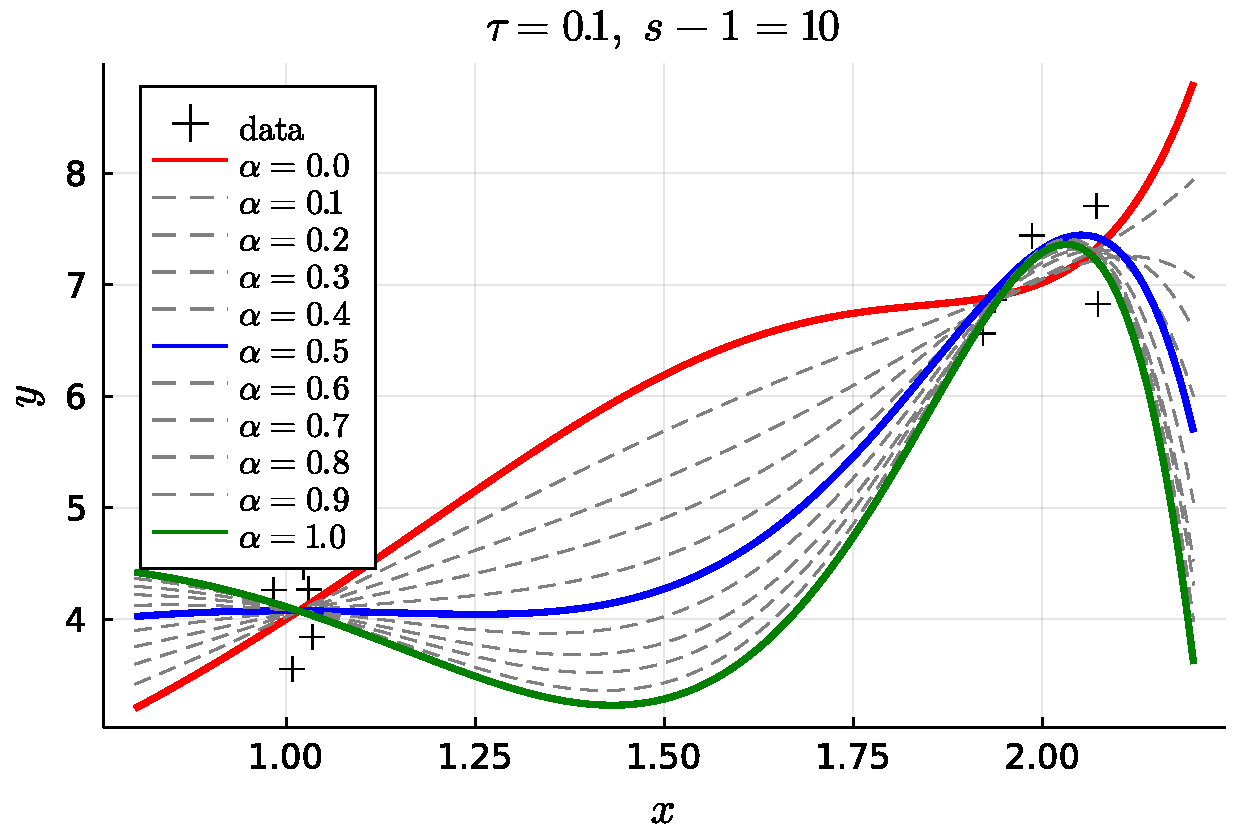
\includegraphics[width=8.0cm]{plots/Images/tau01.pdf} }}%
	\subfloat[Estimated model for $\tau=10$ and $s=11$.]
	{{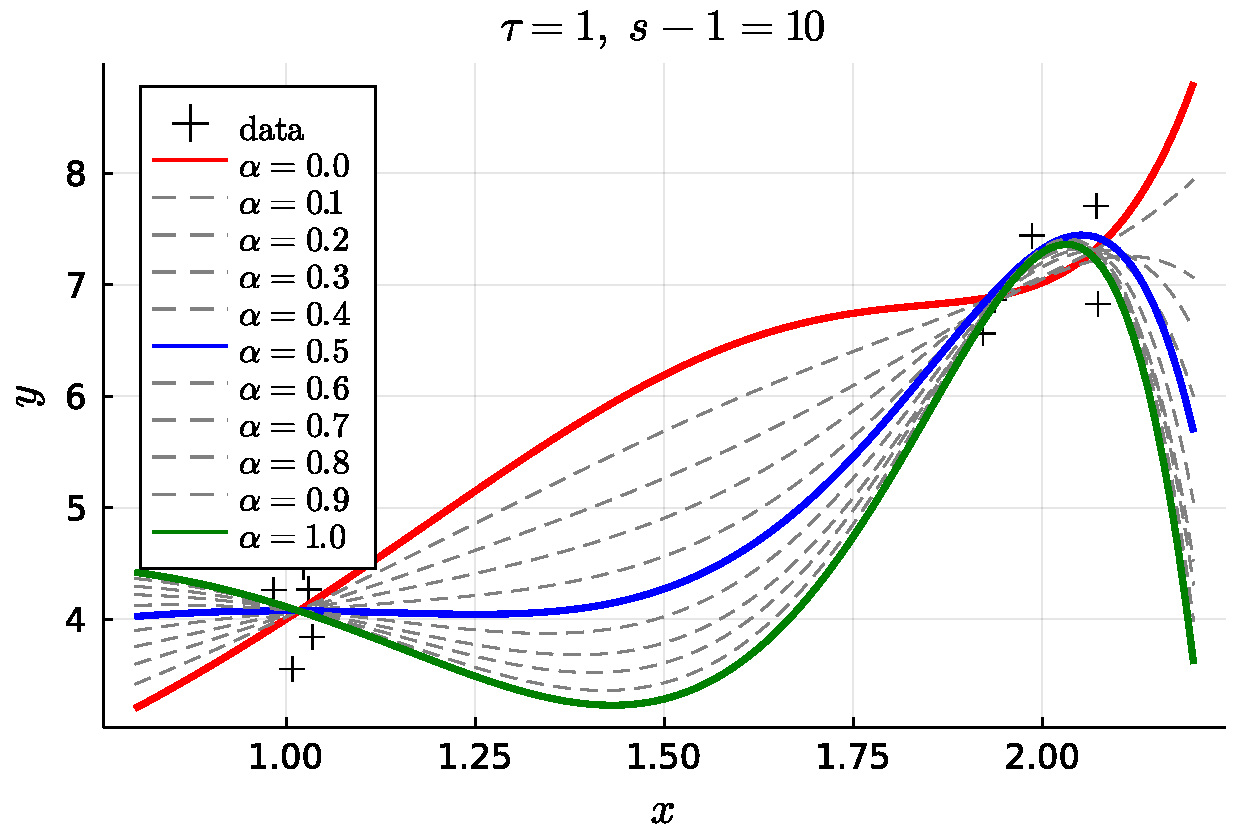
\includegraphics[width=8.0cm]{plots/Images/tau1.pdf} }}%
	\
	\subfloat[Estimated model for $\tau=100$ and $s=11$.]
	{{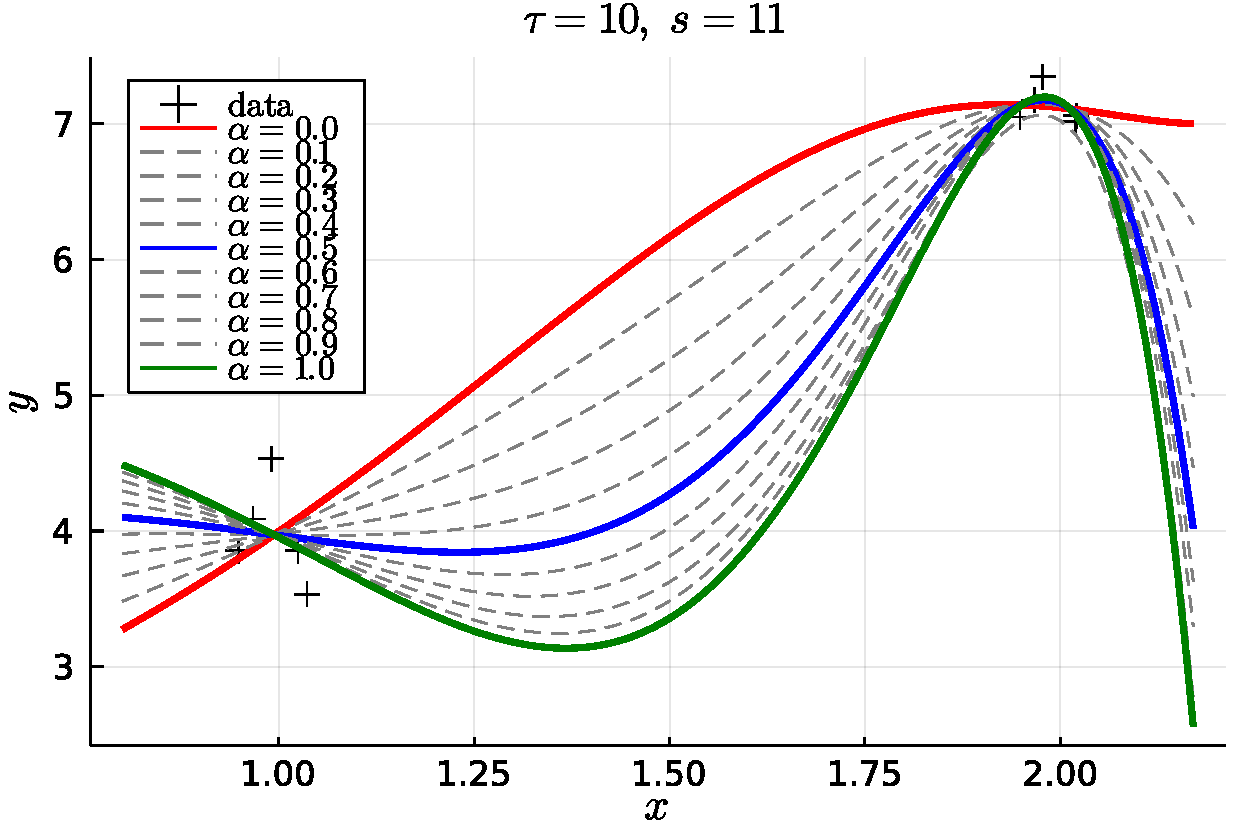
\includegraphics[width=8.0cm]{plots/Images/tau10.pdf} }}%,
	\subfloat[Estimated model for $\tau=1000$ and $s=11$.]
	{{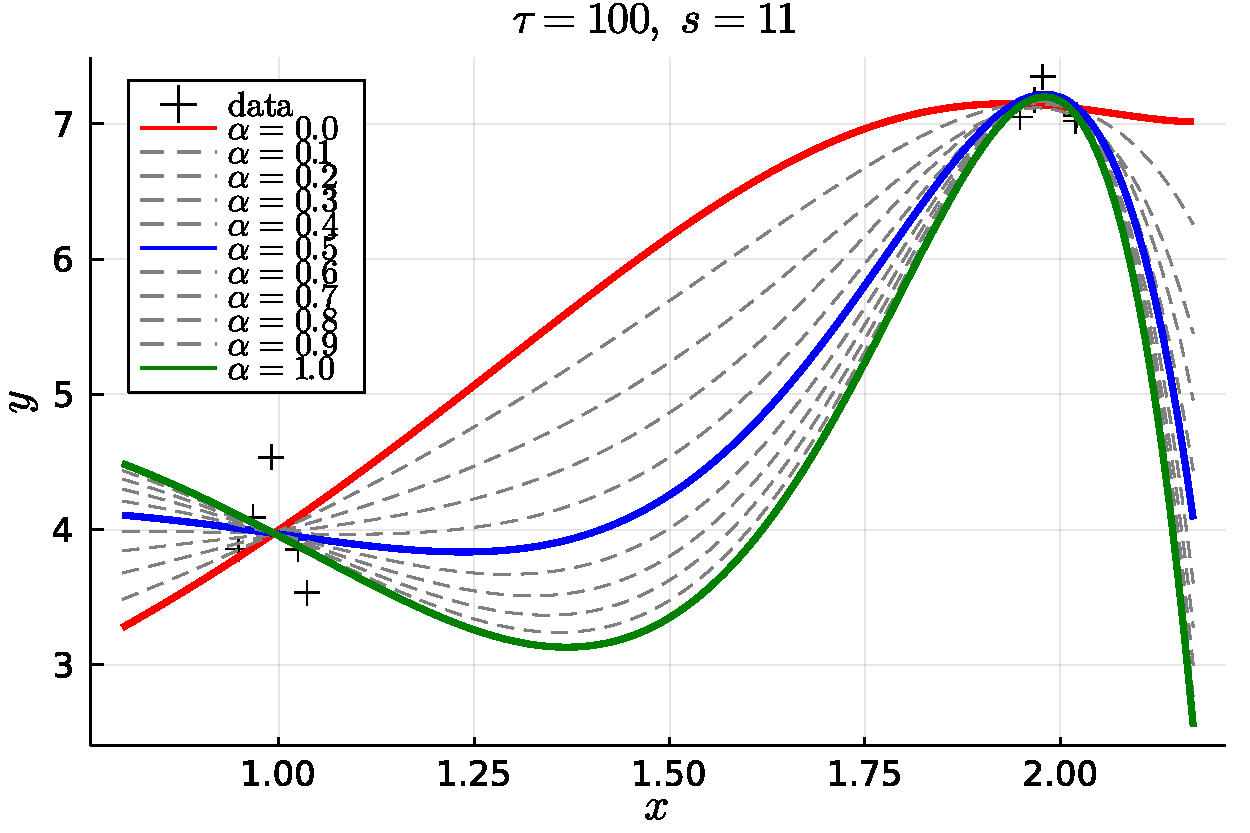
\includegraphics[width=8.0cm]{plots/Images/tau100.pdf} }}%
	\
	\subfloat[Estimated model for $\tau=100000$ and $s=11$.]
	{{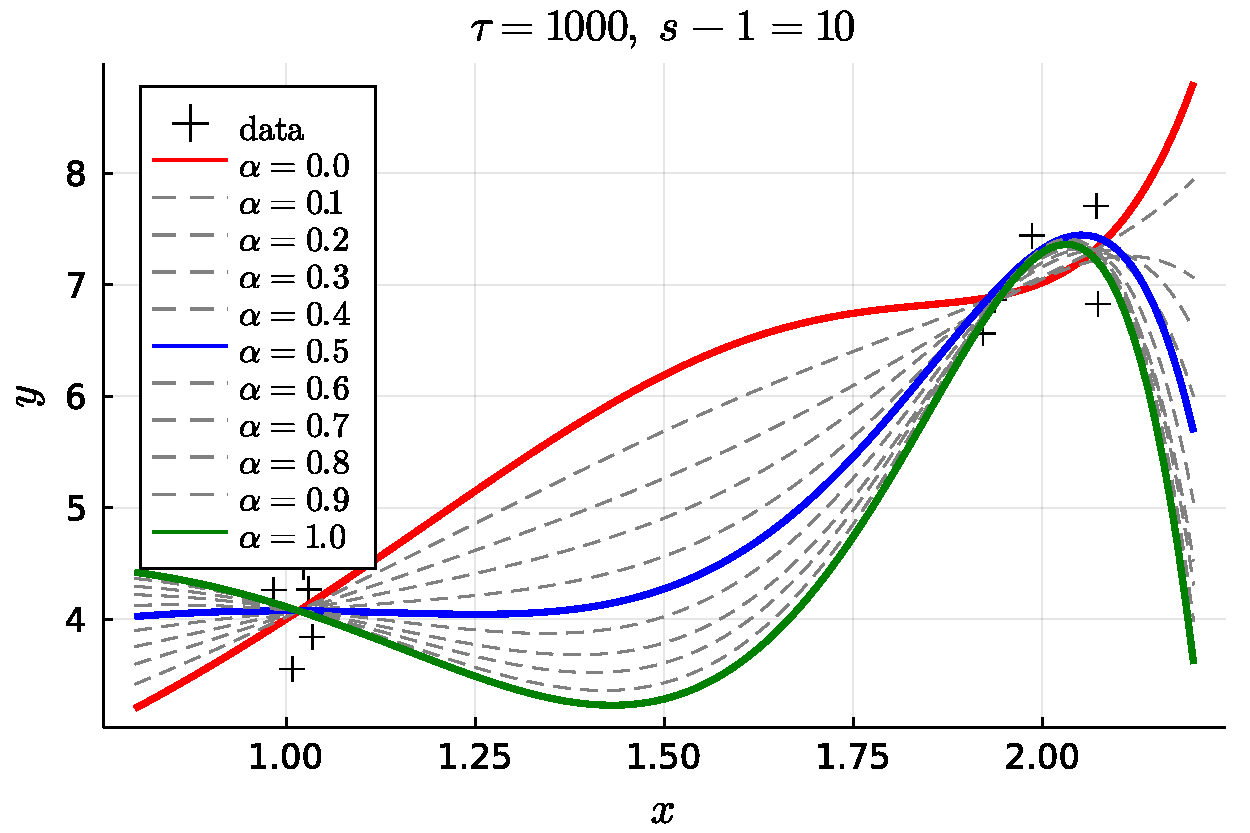
\includegraphics[width=8.0cm]{plots/Images/tau1000.pdf} }}%,
	\subfloat[Estimated model for $\tau=1000000$ and $s=11$.]
	{{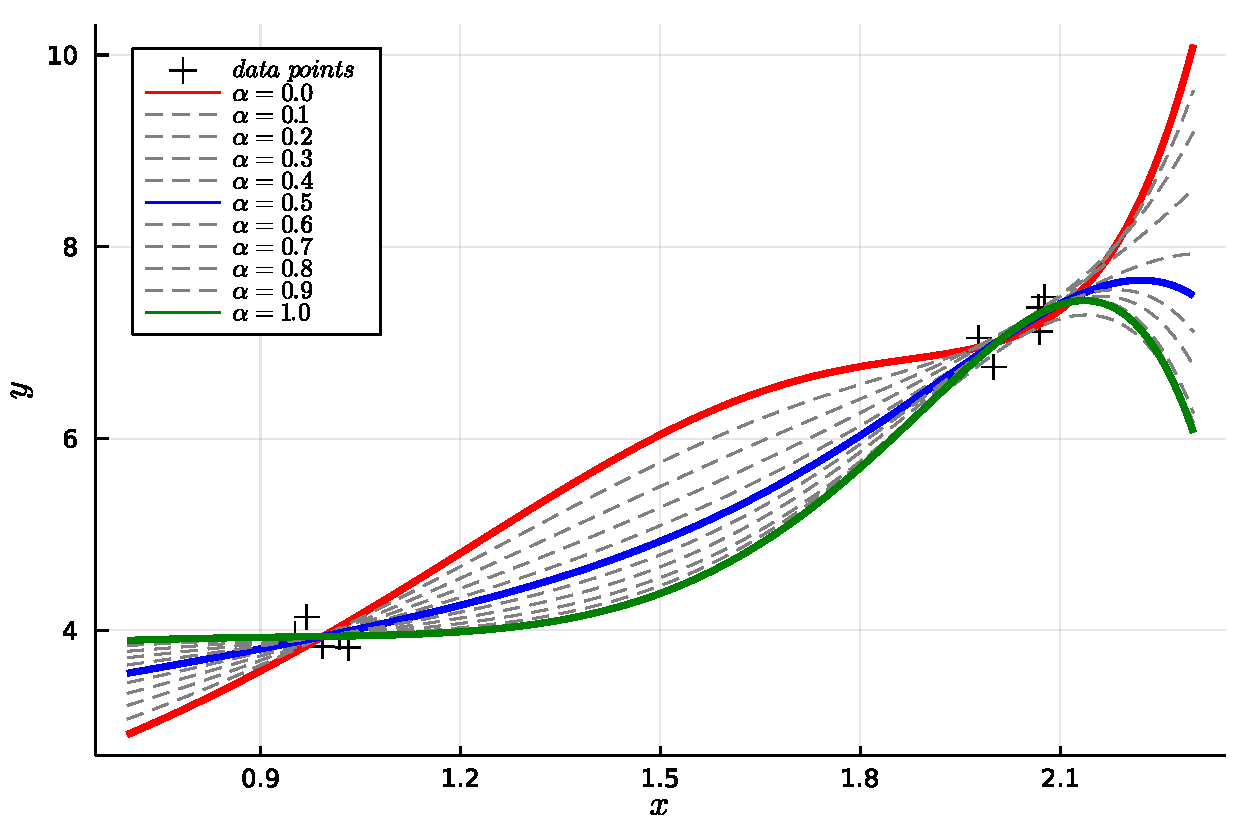
\includegraphics[width=8.0cm]{plots/Images/tau10000.pdf} }}%
	\caption{Sensitivity of the polynomial model to parameter $\tau$ with parameter $s-1$ held fixed for six different cases.}%
	\label{fig:linregtoy_tau}%
\end{figure}

\begin{figure}[h]
	\centering
	\subfloat[Estimated model for $\tau=100$ and $s-1=2$.]
	{{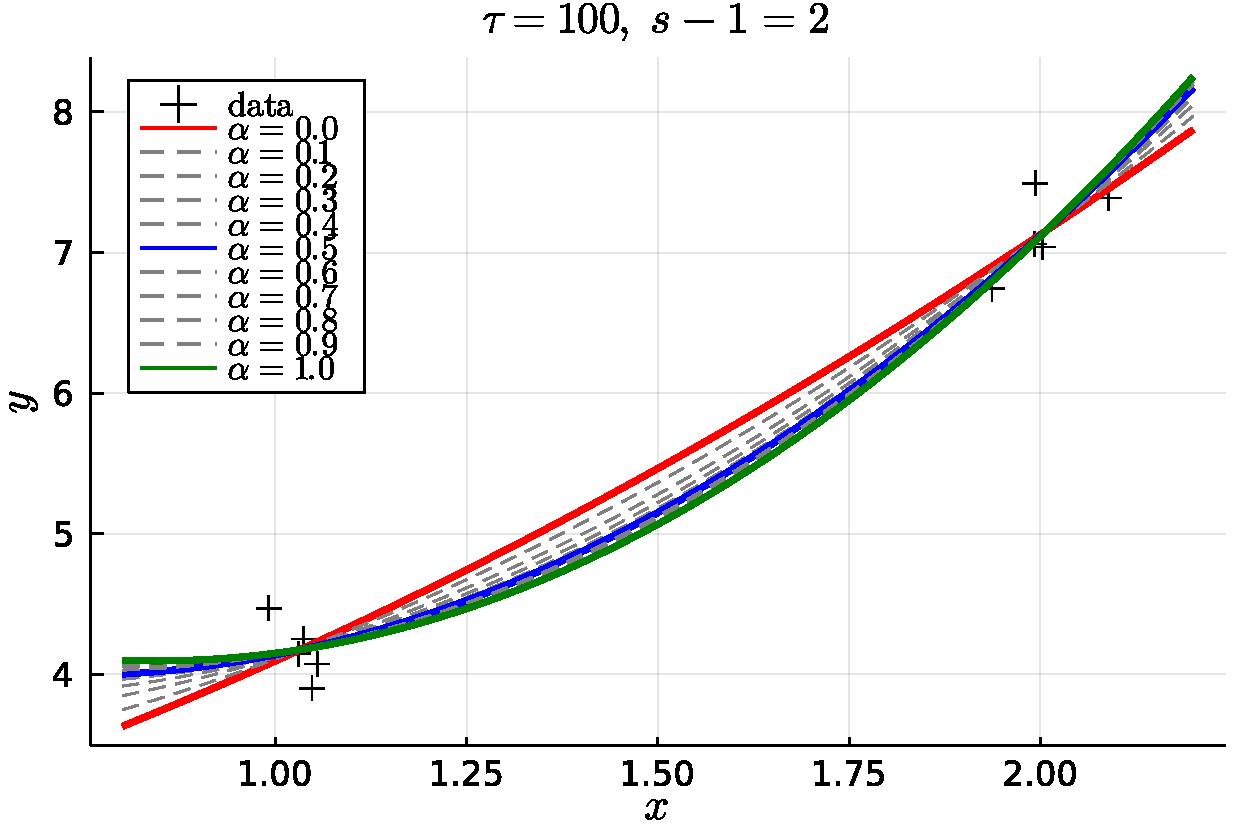
\includegraphics[width=8.0cm]{plots/Images/n2.pdf} }}%
	\subfloat[Estimated model for $\tau=100$ and $s-1=4$.]
	{{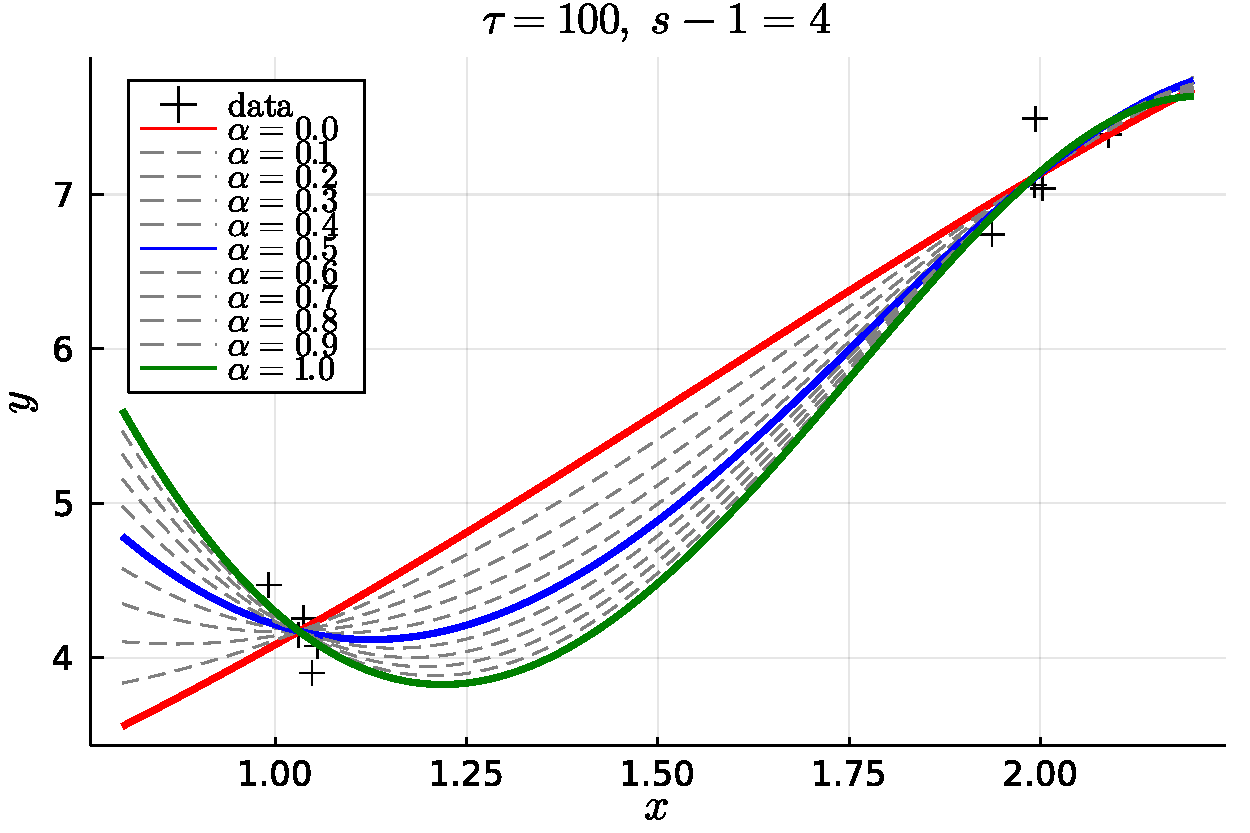
\includegraphics[width=8.0cm]{plots/Images/n4.pdf} }}%
	\
	\subfloat[Estimated model for $\tau=100$ and $s-1=5$.]
	{{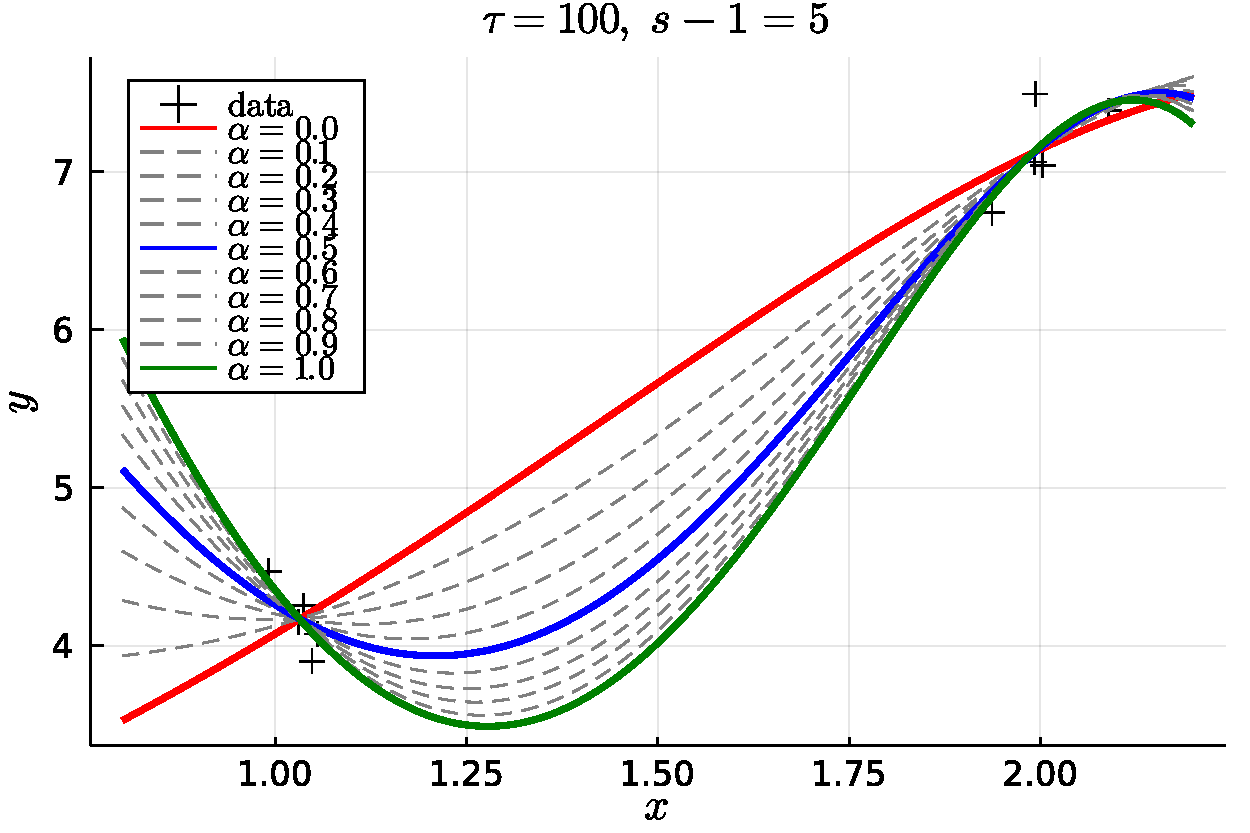
\includegraphics[width=8.0cm]{plots/Images/n5.pdf} }}%,
	\subfloat[Estimated model for $\tau=100$ and $s-1=6$.]
	{{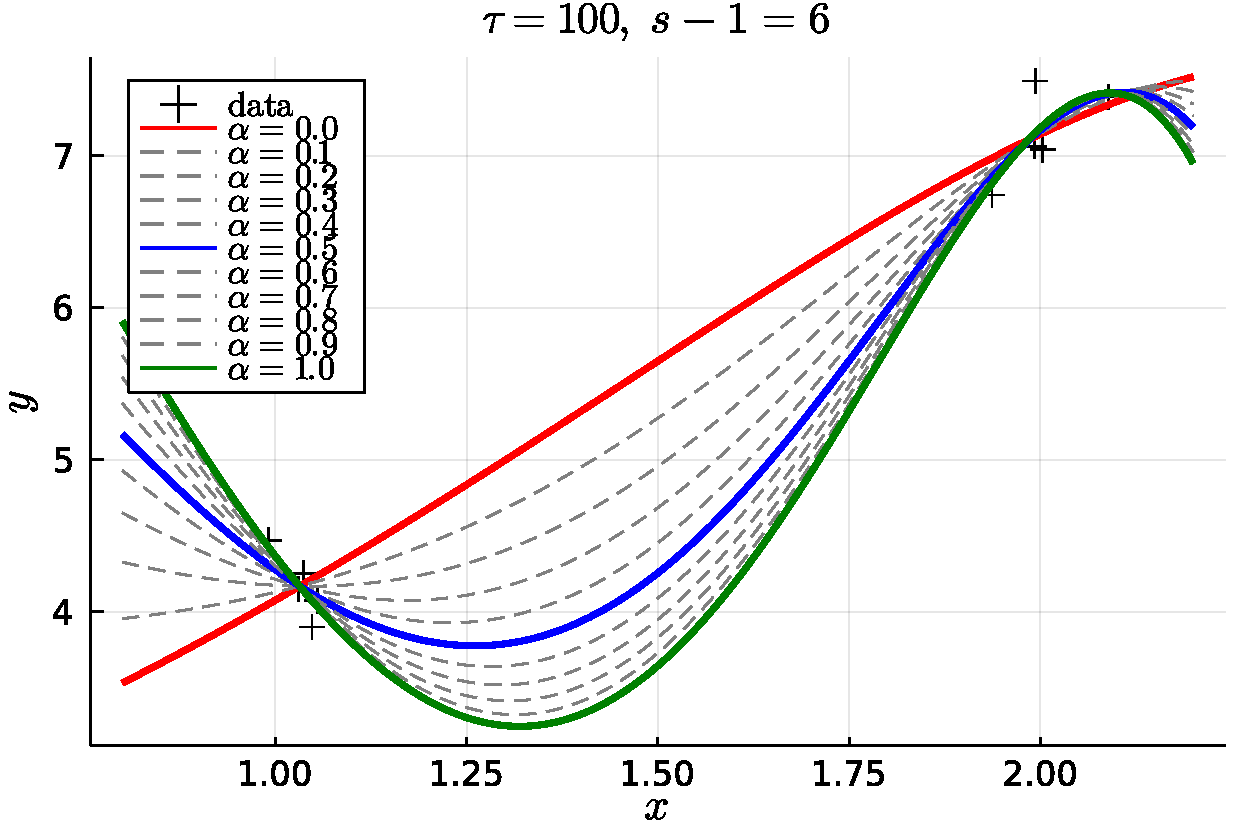
\includegraphics[width=8.0cm]{plots/Images/n6.pdf} }}%
	\
	\subfloat[Estimated model for $\tau=100$ and $s-1=8$.]
	{{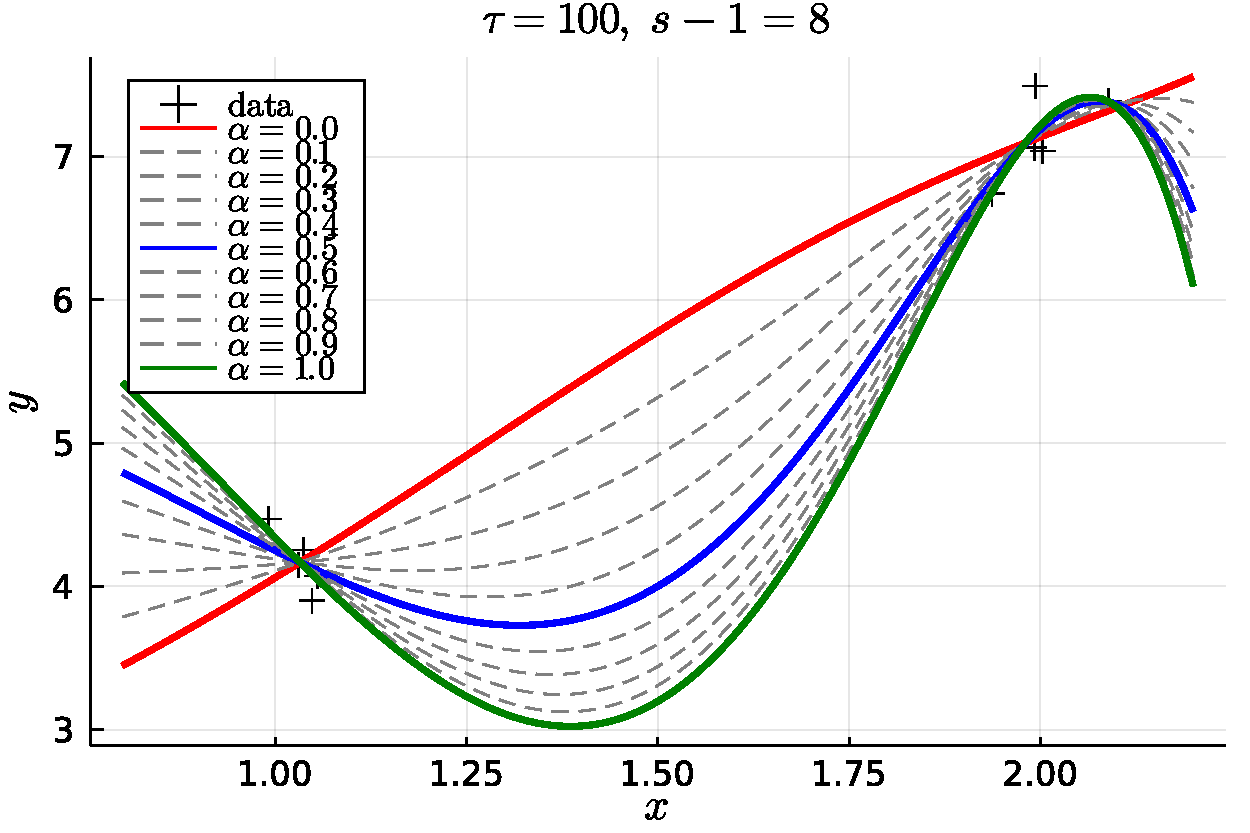
\includegraphics[width=8.0cm]{plots/Images/n8.pdf} }}%,
	\subfloat[Estimated model for $\tau=100$ and $s-1=10$.]
	{{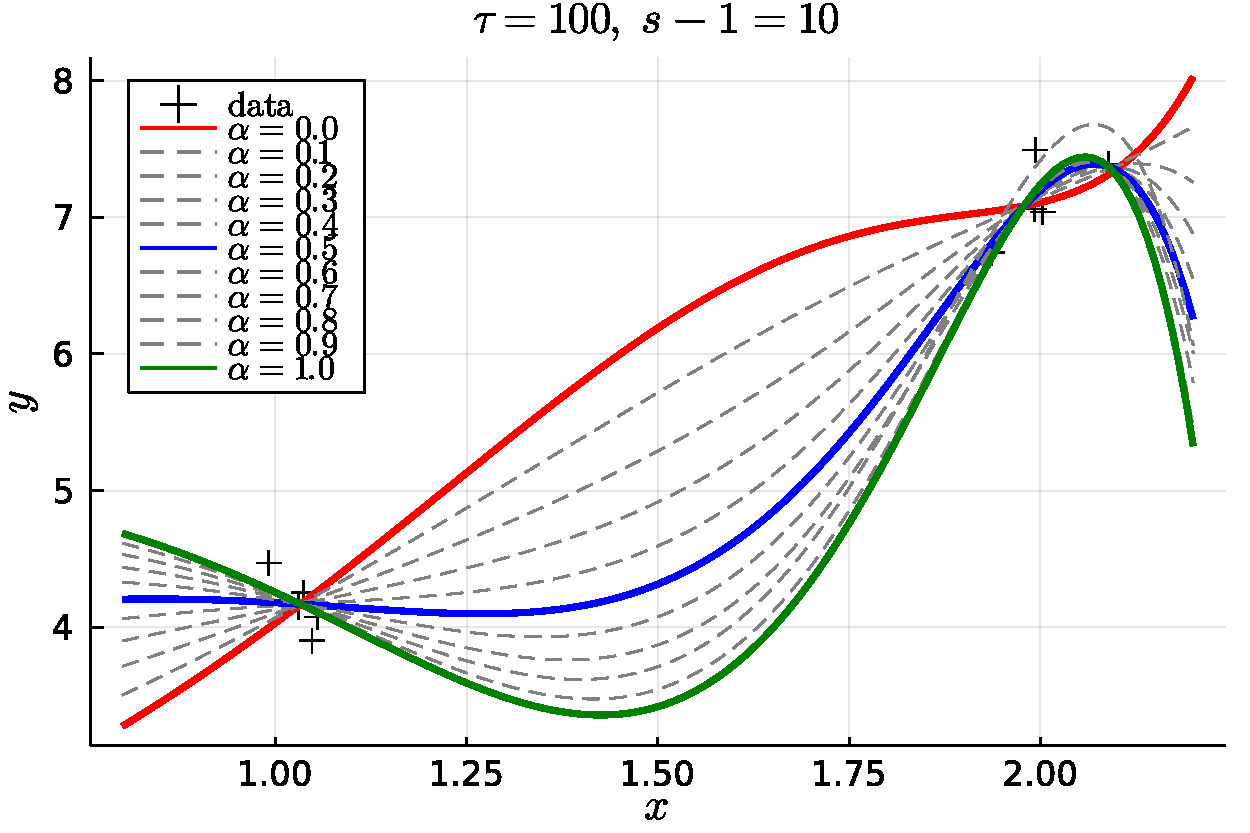
\includegraphics[width=8.0cm]{plots/Images/n10.pdf} }}%
	\caption{Sensitivity of the polynomial model to the order of polynomial $s-1$ for six different cases.}%
	\label{fig:linregtoy_s}%
\end{figure}